% ****** Start of file apssamp.tex ******
%
%   This file is part of the APS files in the REVTeX 4.1 distribution.
%   Version 4.1r of REVTeX, August 2010
%
%   Copyright (c) 2009, 2010 The American Physical Society.
% 
%   See the REVTeX 4 README file for restrictions and more information.
%
% TeX'ing this file requires that you have AMS-LaTeX 2.0 installed
% as well as the rest of the prerequisites for REVTeX 4.1
%
% See the REVTeX 4 README file
% It also requires running BibTeX. The commands are as follows:
%
%  1)  latex apssamp.tex
%  2)  bibtex apssamp
%  3)  latex apssamp.tex
%  4)  latex apssamp.tex
%
\documentclass[%
reprint,
superscriptaddress,
%groupedaddress,
%unsortedaddress,
%runinaddress,
%frontmatterverbose, 
% preprint,
%showpacs,preprintnumbers,
%nofootinbib,
%nobibnotes,
%bibnotes,
amsmath,amssymb,
aps,
prl,
%pra,
% prb,
%rmp,
%prstab,
%prstper,
%floatfix,
]{revtex4-1}

\usepackage{array}
\usepackage{graphicx}% Include figure files
\usepackage{dcolumn}% Align table columns on decimal point
\usepackage{bm}% bold math
\usepackage{amsmath}
%\usepackage{hyperref}% add hypertext capabilities
%\usepackage[mathlines]{lineno}% Enable numbering of text and display math
%\linenumbers\relax % Commence numbering lines

%\usepackage[showframe,%Uncomment any one of the following lines to test 
%%scale=0.7, marginratio={1:1, 2:3}, ignoreall,% default settings
%%text={7in,10in},centering,
%%margin=1.5in,
%%total={6.5in,8.75in}, top=1.2in, left=0.9in, includefoot,
%%height=10in,a5paper,hmargin={3cm,0.8in},
%]{geometry}

% % https://tex.stackexchange.com/questions/231191/algorithm-in-revtex4-1
\usepackage{algorithm}
\usepackage{algpseudocode}


\begin{document}

\title{Active Learning of Atomistic Force Fields}

\author{Jonathan Vandermause}
\affiliation{Department of Physics, Harvard University, Cambridge, MA 02138, USA}
\affiliation{John A. Paulson School of Engineering and Applied
Sciences, Harvard University, Cambridge, MA 02138, USA}

\author{Steven B. Torrisi}
\affiliation{Department of Physics, Harvard University, Cambridge, MA 02138, USA}

\author{Simon Batzner}
\affiliation{Center for Computational Engineering, Massachusetts Institute of Technology, Cambridge, MA 02139, USA}

\author{Boris Kozinsky}
\affiliation{John A. Paulson School of Engineering and Applied
Sciences, Harvard University, Cambridge, MA 02138, USA}


% \author{Jonathan Vandermause,$^{1,2}$ Steven B. Torrisi,$^{2}$
%     Simon Batzner,$^{3}$ Alexie Kolpak,$^{4}$ and Boris Kozinsky$^{1}$}
% \affiliation{$^{1}$John A. Paulson School of Engineering and Applied
% Sciences, Harvard University, Cambridge, Massachusetts 02138, USA \\
% $^{2}$Department of Physics, Harvard University, Cambridge, Massachusetts
% 02138, USA \\
% $^{3}$Center for Computational Engineering, Massachusetts Institute of
% Technology, Cambridge, Massachusetts 02139, USA \\
% $^{4}$ Department of Mechanical Engineering, Massachusetts Institute of Technology, Cambridge, Massachusetts 02139, USA}

\date{\today}

\begin{abstract}
\textit{Ab initio} molecular dynamics is a powerful tool for
accurately probing the dynamics of molecules and solids, but it is limited
to system sizes on the order of 1000 atoms and time scales on the order of
10 ps. We present a scheme for rapidly training a machine learning 
model of the interatomic force field that approaches the accuracy of \textit{ab initio} force calculations but can be applied to larger systems over longer time scales. Gaussian Process models are trained “on-the-fly”, with density-functional theory calculations of the atomic forces performed whenever the model encounters chemical configurations outside of the training set. We demonstrate the flexibility of our approach by testing it on vacancy diffusion in bulk metals.
\end{abstract}

\maketitle


\begin{figure}
	\centering
	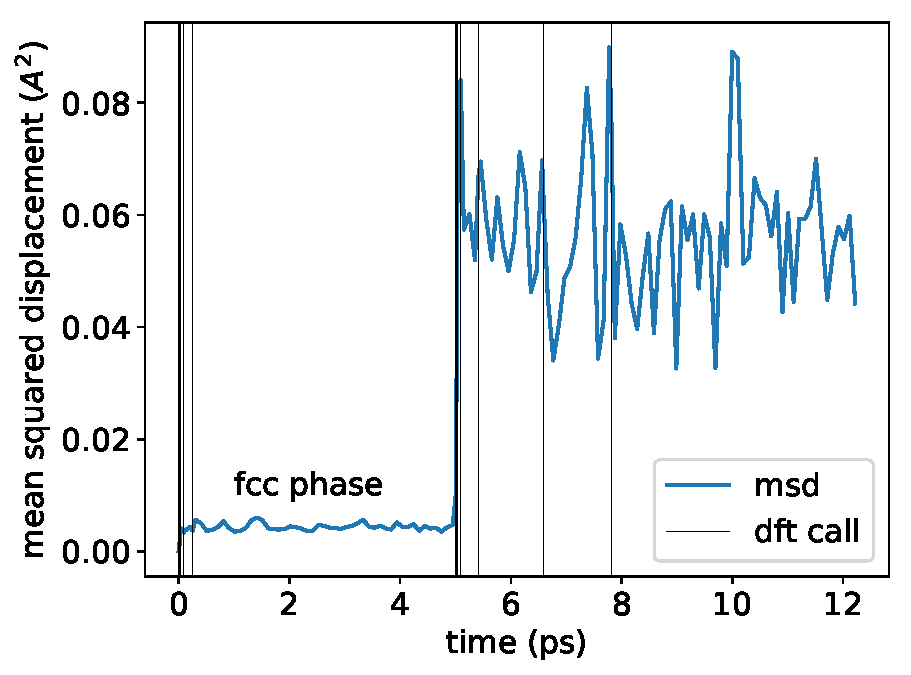
\includegraphics[width=3.4in]{melt_msd.pdf}
	\caption{Mean square displacement of aluminum quench.}
\end{figure}

\begin{figure}
	\centering
	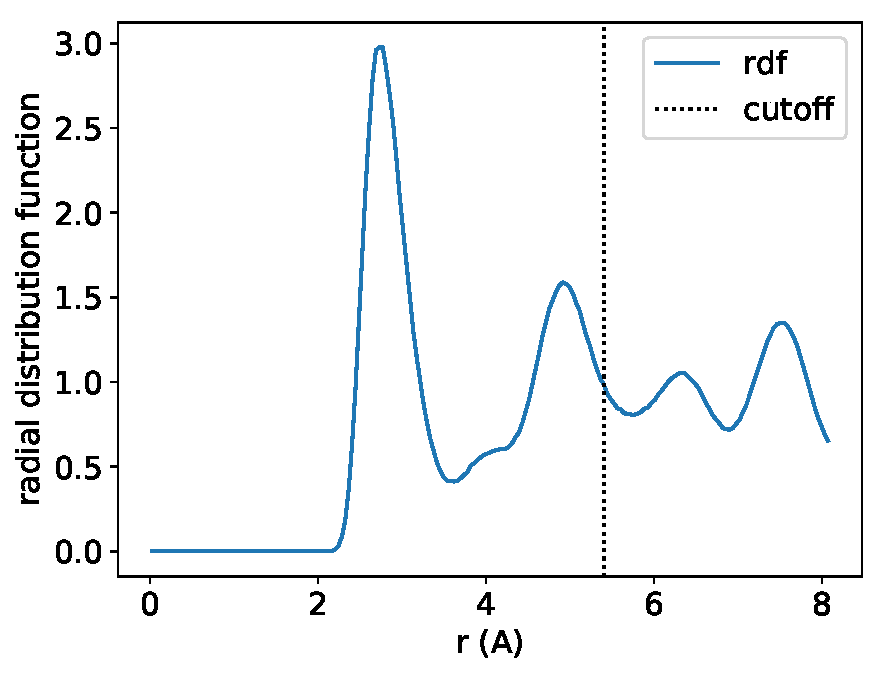
\includegraphics[width=3.4in]{rdf.pdf}
	\caption{RDF of Al quench.}
\end{figure}

% https://en.wikibooks.org/wiki/LaTeX/Tables
\begin{table}
\begin{tabular}
{ |p{1.4cm}|| >{\centering} p{1.4cm}| >{\centering} p{1.4cm}| >{\centering} p{1.4cm}| p{1.4cm} <{\centering}|  }
	% \hline
	% \multicolumn{4}{|c|}{Model Error} \\
	\hline
	 & Solid & Liquid & Slab & Vacancy \\
	\hline
	OTF & \bf{test} & & & \\
	\hline
	EAM & & & & \\
	\hline
\end{tabular}
\caption{On-the-fly force field error compared to a recent EAM potential.}
\end{table}

% https://en.wikibooks.org/wiki/LaTeX/Algorithms#Typesetting_using_the_algorithmic_package
\begin{algorithm}[H]
  \caption{Active Learning of Atomistic Force Fields}
  \label{EPSA}
   \begin{algorithmic}[1]
   \Require initial structure (positions, velocities, periodic cell)
   \Require initial GP model (kernel and hyperparameters)
   \Require $\Delta t$: molecular dynamics time step
   \Require $T$: total simulation time
   \Require $\mathcal{U}$: initial uncertainty threshold
   \State Initialize time: t = 0
   \While {$t < T$}
   \State predict forces and uncertainties with GP model
   \If {uncertainty above threshold}
   \State compute forces with DFT
   \State add highest uncertainty atom to training set
   \State update GP hyperparameters
   \State update structure with DFT forces
   \Else
   \State update structure with GP forces
   \EndIf
   \State update time: $t = t + \Delta t$
   \EndWhile
   \end{algorithmic}
\end{algorithm}


% \section{Literature}
% \begin{enumerate}

% \item On-the-fly force fields with GPs and KRR \cite{li2015molecular, botu2015adaptive, botu2015learning}

% \item Gaussian Approximation Potentials (GAP)
% \cite{bartok2010gaussian, bartok2015gaussian, deringer2017machine}

% \item The SOAP kernel \cite{bartok2013representing}

% \item Other covariant kernels (two- and three-body) \cite{deringer2017machine, bartok2015gaussian, glielmo2017accurate, glielmo2018efficient}

% \item Vector-valued GPs and ICM \cite{alvarez2012kernels}

% \item DFT and Quantum Espresso \cite{kohn1999nobel, giannozzi2009quantum}

% \end{enumerate}

% \section{Smooth two-body kernel}
% We find that a covariant two-body kernel gives good accuracy for bulk metals with a vacancy \cite{glielmo2018efficient, deringer2017machine}. The covariant kernel implemented here is derived from a rotationally invariant local energy kernel $k_{\text{inv}}$ that directly compares interatomic distances:
% \begin{equation}
% k_{\text{inv}} = \sigma^2 \sum_{i ,j} \exp\left( - \frac{(r_i - r_j)^2}{2 \ell^2} \right) f_{\text{cut}}(r_i) f_{\text{cut}}(r_j),
% \label{loc_kern}
% \end{equation}
% where the sum ranges over all atoms in the atomic environments. $f_{\text{cut}}$ is a cutoff function that ensures that the local energy and its derivative go smoothly to zero at finite radius $r_{\text{cut}}$ \cite{bartok2015gaussian}:
% \begin{equation}
% f_{\text{cut}} =  \begin{cases} 
%     1 & r\leq r_{\text{cut}}-d, \\
%     \frac{\cos(\pi \frac{r-r_{\text{cut}}+d}{d}) + 1}{2} & r_{\text{cut}} - d < r \le r_{\text{cut}}, \\
%     0 & r > r_{\text{cut}}.
%  \end{cases}
% \end{equation}
% The cutoff function smooths the model by eliminating sharp discontinuities associated with atoms entering and leaving the cutoff sphere surrounding the central atom.

% The local energy kernel described by Eq.\ (\ref{loc_kern}) induces a covariant matrix-valued force kernel $\frac{\partial^2 k_{\text{inv}}}{\partial \xi_i \partial \chi_j}$ suitable for the direct prediction of atomic forces, where $\xi_i$ and $\chi_i$ denote the $i^{\text{th}}$ Cartesian coordinate of the central atom of the first and second atomic environments, respectively. In the table below, we summarize all the terms needed to efficiently calculate the force kernel and its derivatives with respect to the model hyperparameters $\ell, \sigma,$ and $d$.

% \begin{center}
%     \begin{table}
%     \begin{tabular}{ |c|c|c| } 
%      \hline
%      Energy Kernel & $k_{\text{inv}}(\rho_1, \rho_2; \ell, \sigma, d)$ & $\sigma^2 \sum_{i ,j} k(r_i, r_j) f_{\text{cut}}(r_i) f_{\text{cut}}(r_j)$ \\ 
%      \hline
%      - & $k(r_i, r_j; \ell)$ & $\exp\left( - \frac{(r_i - r_j)^2}{2 \ell^2} \right)$\\
%      \hline
%      - & $f_{\text{cut}}(r; d)$ & $\frac{\cos(\pi \frac{r-r_{\text{cut}}+d}{d}) + 1}{2}, \text{ } r_{\text{cut}} - d < r \le r_{\text{cut}}$ \\
%      \hline
%     Force Kernel & $\frac{\partial^2 k_{\text{inv}}}{\partial \xi_i \partial \chi_j}$ & $\sigma^2 \sum_{i ,j} (k_0 + k_1 + k_2 + k_3)$ \\ 
%      \hline
%      - & $k_0(r_i, r_j; \ell, d)$ & $k \frac{\partial f_{\text{cut}}(r_i)}{\partial \xi_i} \frac{\partial f_{\text{cut}}(r_j)}{\partial \chi_j}$ \\ 
%      \hline
%      - & $k_1(r_i, r_j; \ell, d)$ & $\frac{\partial k}{\partial \xi_i} f_{\text{cut}}(r_i) \frac{\partial f_{\text{cut}}(r_j)}{\partial \chi_j}$ \\ 
%      \hline
%      - & $k_2(r_i, r_j; \ell, d)$ & $\frac{\partial k}{\partial \chi_j} \frac{\partial f_{\text{cut}}(r_i)}{\partial \xi_i} f_{\text{cut}}(r_j)$ \\ 
%      \hline
%      - & $k_3(r_i, r_j; \ell, d)$ & $\frac{\partial^2 k}{\partial \xi_i \partial \chi_j} f_{\text{cut}}(r_i) f_{\text{cut}}(r_j)$ \\ 
%      \hline
%      - & $\frac{\partial k}{\partial \xi_i}$ & $\frac{k (r_i-r_j) \xi_i}{\ell^2 r_i}$ \\ 
%      \hline
%      - & $\frac{\partial k}{\partial \chi_j}$ & $\frac{k (r_j-r_i) \chi_j}{\ell^2 r_j}$ \\ 
%      \hline
%      - & $\frac{\partial^2 k}{\partial \xi_i \chi_j}$ & $\frac{k \xi_i \chi_j (\ell^2 - (r_j-r_i)^2)}{\ell^4 r_i r_j}$ \\ 
%      \hline
%      - & $\frac{\partial f_\text{cut}(r_i)}{\partial \xi_i}$ & $ \frac{\pi \xi_i}{2d r_i} \sin(\pi \frac{r_{\text{cut}}-r_i}{d}), \text{ } r_{\text{cut}} - d < r \le r_{\text{cut}}$ \\ 
%      \hline
%      $\ell$ Derivative & $\frac{\partial^3 k_{\text{inv}}}{\partial \ell \partial \xi_i \partial \chi_j}$ & $\sigma^2 \sum_{i ,j} \left(\frac{\partial k_0}{\partial \ell} + \frac{\partial k_1}{\partial \ell} + \frac{\partial k_2}{\partial \ell} + \frac{\partial k_3}{\partial \ell}\right)$ \\
%      \hline
%      - & $\frac{\partial k}{\partial \ell}$ & $\frac{k (r_i-r_j)^2}{l^3}$ \\
%      \hline
%      - & $\frac{\partial^2 k}{\partial \ell \partial \xi_i}$ & $\frac{k \xi_i (-2 \ell^2 + (r_i-r_j)^2) (r_i-r_j)}{l^5 r_i}$ \\
%      \hline
%      - & $\frac{\partial^2 k}{\partial \ell \partial \xi_i \partial \chi_j}$ & $\frac{k \xi_i \chi_j \left(-2 \ell^4 + 5 \ell^2 (r_i-r_j)^2 - (r_i-r_j)^4 \right)}{l^7 r_i r_j}$ \\
%      \hline
%      $d$ Derivative & $\frac{\partial f_{\text{cut}}(r_i)}{\partial d}$ & $\frac{\pi (r-r_{\text{cut}})}{2 d^2} \sin\left( \frac{\pi (r_{\text{cut}} - r)}{d} \right)$ \\
%      \hline
%      - & $\frac{\partial^2 f_{\text{cut}}(r_i)}{\partial d \partial \xi_i}$ & $\frac{\pi \xi_i \left( \pi (r - r_{\text{cut}}) \cos \left( \frac{\pi (r - r_{\text{cut}})}{d} \right) + d \sin \left( \frac{\pi (r-r_{\text{cut}})}{d} \right) \right)}{2 d^3 r_i}$\\
%      \hline
%      $\sigma$ Derivative & $\frac{\partial^3 k_{\text{inv}}}{\partial \sigma \partial \xi_i \partial \chi_j}$ & $2 \sigma \sum_{i ,j} (k_0 + k_1 + k_2 + k_3)$ \\
%      \hline
%     \end{tabular}
%     \caption{Quantities used to calculate the smoothed two-body force kernel and its derivatives.}
% \end{table}
% \end{center}

\begin{center}
    \begin{table}
    \begin{tabular}{ |c|c|c| } 
     \hline
     Energy Kernel & $k_{\text{inv}}$ & $\sigma^2 \sum_{c, p} k f_{\text{cut}}(\vec{d}_c) f_{\text{cut}}(\vec{d}_p)$ \\ 
     \hline
     - & $k$ & $\exp\left( - \frac{||\vec{d}_c - \vec{d}_p ||^2}{2 \ell^2} \right)$\\
     \hline
     - & $\vec{d}^{(2)}$ & $(r_{i_1})$ \\
     \hline
     - & $\vec{d}^{(3)}$ & $(r_{i_1}, r_{i_2}, r_{i_1, i_2})$ \\
     \hline
    Force Kernel & $\frac{\partial^2 k_{\text{inv}}}{\partial \xi_i \partial \chi_j}$ & $\sigma^2 \sum_{c, p} (k_0 + k_1 + k_2 + k_3)$ \\ 
     \hline
     - & $k_0$ & $k \frac{\partial f_{\text{cut}}(\vec{d}_c)}{\partial \xi_i} \frac{\partial f_{\text{cut}}(\vec{d}_p)}{\partial \chi_j}$ \\ 
     \hline
     - & $k_1$ & $\frac{\partial k}{\partial \xi_i} f_{\text{cut}}(\vec{d}_c) \frac{\partial f_{\text{cut}}(\vec{d}_p)}{\partial \chi_j}$ \\ 
     \hline
     - & $k_2$ & $\frac{\partial k}{\partial \chi_j} \frac{\partial f_{\text{cut}}(\vec{d}_c)}{\partial \xi_i} f_{\text{cut}}(\vec{d}_p)$ \\ 
     \hline
     - & $k_3$ & $\frac{\partial^2 k}{\partial \xi_i \partial \chi_j} f_{\text{cut}}(\vec{d}_c) f_{\text{cut}}(\vec{d}_p)$ \\ 
     \hline
     - & $\frac{\partial k}{\partial \xi_i}$ & $\frac{k B_1}{\ell^2}$ \\ 
     \hline
     & $B_1$ & $\sum_{q=1}^{N-1} \frac{(r_{i_q} - r_{j_q})\xi_{i_q}}{r_{i_q}}$ \\
     \hline
     - & $\frac{\partial k}{\partial \chi_j}$ &  $-\frac{k B_2}{\ell^2}$ \\ 
     \hline
    - & $B_2$ & $\sum_{q=1}^{N-1} \frac{(r_{i_q} - r_{j_q})\chi_{j_q}}{r_{j_q}}$ \\
     \hline
     - & $\frac{\partial^2 k}{\partial \xi_i \chi_j}$ & $\frac{k}{\ell^4} \left(A \ell^2 -B_1 B_2 \right)$\\ 
     \hline
     - & $A$ & $\sum \frac{\xi_{i_q} \chi_{j_q}}{r_{i_q} r_{j_q}}$ \\
     \hline
     $\ell$ Derivative & $\frac{\partial^3 k_{\text{inv}}}{\partial \ell \partial \xi_i \partial \chi_j}$ & $\sigma^2 \sum_{c, p} \left(\frac{\partial k_0}{\partial \ell} + \frac{\partial k_1}{\partial \ell} + \frac{\partial k_2}{\partial \ell} + \frac{\partial k_3}{\partial \ell}\right)$ \\
     \hline
     - & $\frac{\partial k}{\partial \ell}$ & $\frac{k ||\vec{d}_c - \vec{d}_p||^2}{l^3}$ \\
     \hline
     - & $\frac{\partial^2 k}{\partial \ell \partial \xi_i}$ & $B_1 \left( \frac{1}{\ell^2} \frac{\partial k}{\partial \ell} - \frac{2 k}{\ell^3} \right)$ \\
     \hline
     - & $\frac{\partial^2 k}{\partial \ell \partial \chi_j}$ & $-B_2 \left( \frac{1}{\ell^2} \frac{\partial k}{\partial \ell} - \frac{2 k}{\ell^3} \right)$ \\
     \hline
     - & $\frac{\partial^3 k}{\partial \ell \partial \xi_i \partial \chi_j}$ & $\left( A \ell^2 - B_1 B_2 \right) \left( \frac{\partial k}{\partial \ell} \frac{1}{\ell^4} - \frac{4 k}{\ell^5} \right) + \frac{2 k A}{\ell^3}$ \\
     \hline
     $\sigma$ Derivative & $\frac{\partial^3 k_{\text{inv}}}{\partial \sigma \partial \xi_i \partial \chi_j}$ & $2 \sigma \sum_{c, p} (k_0 + k_1 + k_2 + k_3)$ \\
     \hline
    \end{tabular}
    \caption{Quantities used to calculate the smoothed $N$-body force kernel and its derivatives.}
\end{table}
\end{center}

% \section{On-the-fly learning}

% \section{Computational details}

% \section{Covariant kernels}

% This section will discuss our approach to modelling multi-species systems.
% \begin{enumerate}
% \item Review our two- and three-body single-component kernels, which are similar to the ones used in \cite{glielmo2018efficient, deringer2017machine}. Our three-body kernel is slightly different from both: \cite{glielmo2018efficient} does not distinguish between cross-bonds and central-bonds, and \cite{deringer2017machine} combines the central-bond lengths in a way that doesn't easily generalize to multi-component systems.

% We should also highlight our approach to selecting the GP hyperparameters, which hasn't been discussed at length in the GAP literature. Our approach maximizes the marginal likelihood, and is therefore data-driven rather than empirical. Optimizing the hyperparameters in this way can reveal interesting physics. For example, in the two-plus-three body kernel,
% \begin{equation}
%     k(\rho_1, \rho_2) = \delta_2 k_2 (\rho_1, \rho_2) + \delta_3 k_3(\rho_1, \rho_2),
% \end{equation}
% the size of the hyperparameters $\delta_2$ and $\delta_3$ indicates the relative importance of two- and three-body interactions in the system.

% There is one ``special" hyperparameter, the cutoff radius, which can't be easily optimized using gradient descent. We should justify our cutoff choice using the ``freeze-and-perturb" method of \cite{deringer2017machine}. This will also give a lower bound on the error of any local ML model, which is a useful benchmark. It might be interesting to compare this lower bound with the noise variance of the model, which is an internal measure of how well the model is able to capture the data.

% It would be nice to benchmark the performance of the two-body, three-body, and two-plus-three body single-component kernels by showing the model performance as a function of training set size for a representative system (e.g. solid-state C at 1000 K). Since the focus of this section is on characterizing and benchmarking the kernel, we can train on a constant-T AIMD trajectory.

% \item Discuss our generalization to multi-component systems. There are three plausible ways of going about this: comparing every bond to every other bond (no distinction between different species, which might make sense for similar atoms); comparing bonds of the same type only (which wastes information by neglecting similarities between different bond types); and weighting each bond pair with a hyperparameter. The third method, which is equivalent to an ICM model, provides a general way to capture covariance between different outputs that should be more accurate than the first approach and more efficient than the second. 

% We can plot model performance versus training set size on a SiC system for each of the three methods mentioned above and for each of the three kernels (two-body, three-body, and two-plus-three body). The two-plus-three body kernel will have a lot of hyperparameters (on the order of 100), but it should be feasible with our gradient descent scheme.
% \end{enumerate}

% \section{On-the-fly learning}
% We've so far come up with three interesting applications that highlight the utility of our on-the-fly program: large systems outside the reach of AIMD, bond formation and bond breaking in molecules, and diffusion in solids. In all examples that we try, it will be important to use the converged force field to predict a physical property (e.g. phonon dispersion, bond length, activation energy) and compare the prediction against the ``exact'' value computed with DFT.

% \begin{enumerate}
% \item Large systems. As a test case, we can consider a simple solid-state example, e.g. a 5000-atom bulk SiC sample, and use the ``punchout" method to train an initial force field. In this approach, an atom is first selected at random, a small cubic cell containing the atom and 20-30 of its neighbors is sent to Quantum Espresso, and the resulting force data is used to build a GP model. The model then loops through the remaining atoms and makes predictions, augmenting the database whenever the uncertainty threshold is reached. Once the model converges, it can be tested by predicting the phonon spectrum of SiC and comparing against DFPT.

% \item Bond formation and bond breaking. The simplest example is on-the-fly modelling of the bond energy of $\text{H}_2$. We might also try more complicated examples: 
% \begin{itemize}
% \item Starting a simulation with separated C and O atoms and allowing bonds to form, comparing the model's predicted bond lengths against bond lengths computed with DFT.
% \item Taking a perturbed benzene molecule and seeing if the model correctly predicts the equilibrium configuration.
% \end{itemize}

% \item Diffusion in solids. Gold diffusing on a silver slab or self-diffusion in bulk aluminum are worth trying. Following \cite{botu2015adaptive, botu2015learning}, once the model has converged, a good test is to predict the potential energy along the migration trajectory by integrating the force field. This energy activation profile can be compared against the corresponding DFT prediction.

% \end{enumerate}


\bibliography{otf.bib}

\end{document}
%
% ****** End of file apssamp.tex ******